\section{Dataset Design}
\subsection{Design Principles}
Personality refers to the combination of characteristics or qualities that form an individual's distinctive character. It encompasses a wide range of traits, behaviors, thoughts, and emotional patterns that evolve from biological and environmental factors~\cite{6406319}. A particular personality can determine various outward observable properties or features, including consistent behavioral patterns, communication style, emotional expression and so on. These traits manifest in how an individual consistently acts and reacts in different situations, their manner of speaking and body language, the openness or restraint of their emotional displays, their ways of relating to others, their approach to making decisions, and their preferences in activities, hobbies, and social engagements.
\subsection{Multiple Personality Models are Needed} 
In constructing such a dataset for personality prediction, incorporating four distinct personality models, provides a comprehensive framework for understanding the multifaceted nature of human Personality. To this end, evolving four distinct personality models—Myers-Briggs Type Indicator (MBTI), Big Five, Enneagram, and Instinctual Variant—into our dataset construction is essential. Each of these models provides a unique lens through which to view and interpret personality traits, offering complementary insights that are critical for a holistic understanding. For instances, MBTI has 16 unique personality types. Among these, INFJ is a personality type with the Introverted, Intuitive, Feeling, and Judging traits. They tend to approach life with deep thoughtfulness and imagination. Their inner vision, personal values, and a quiet, principled version of humanism guide them in all things.
\subsection{Relations to Interpret Personality}

Each personality model offers unique insights and covers different aspects of personality, making them collectively valuable for a multidimensional approach to personality prediction. In addition to these models, we introduce two main categories of relations among characters:

1) \textbf{Social Relations}: These provide a comprehensive framework to observe and interpret the nuances of personality in action. We identify seven types of social relations from the perspectives of psychology and sociology. Based on various social environments, we categorize 7 kinds of social relations including \textit{family, friendship, romantic, professional, social, academic and online}.

2) \textbf{Emotion Relations}: The social relations above are relatively unchangeable, not depicting the attitudes towards someone else. So we define another 8 types for the emotion relations, as the aid for the comprehension of personality. We choose \textit{fondness, jealousy, aversion, pity, respect, hostility, envy and gratitude} as our annotators for the emotional relations, which concludes the diverse attitudes in human's daily life. To annotate these two relations, we select a binary tuple (e.g., \textit{Gil and Adriana: (Romantic, Fondness)}) to represent the relations combination for each pair of characters based on different scenes.

\subsection{Structure of PersonaMovs}
Aiming to deliver a tidy and readable structure, we distribute different scenes in a single text file with corresponding audio and video clip. As shown in Figure \ref{fig:sample}, it provides a timestamp of the scene, a visual snapshot from the movie, and a transcription of their dialogue. The characters' personalities are profiled using various typologies, such as MBTI and Enneagram, with accompanying bar charts showing the distribution of votes or consensus on these personality assessments. Additionally, the relationship between Gatsby and Daisy is categorized as professional with an element of fondness, offering insights into the dynamics of their interaction.

\begin{figure*}[th!]
  \centering
  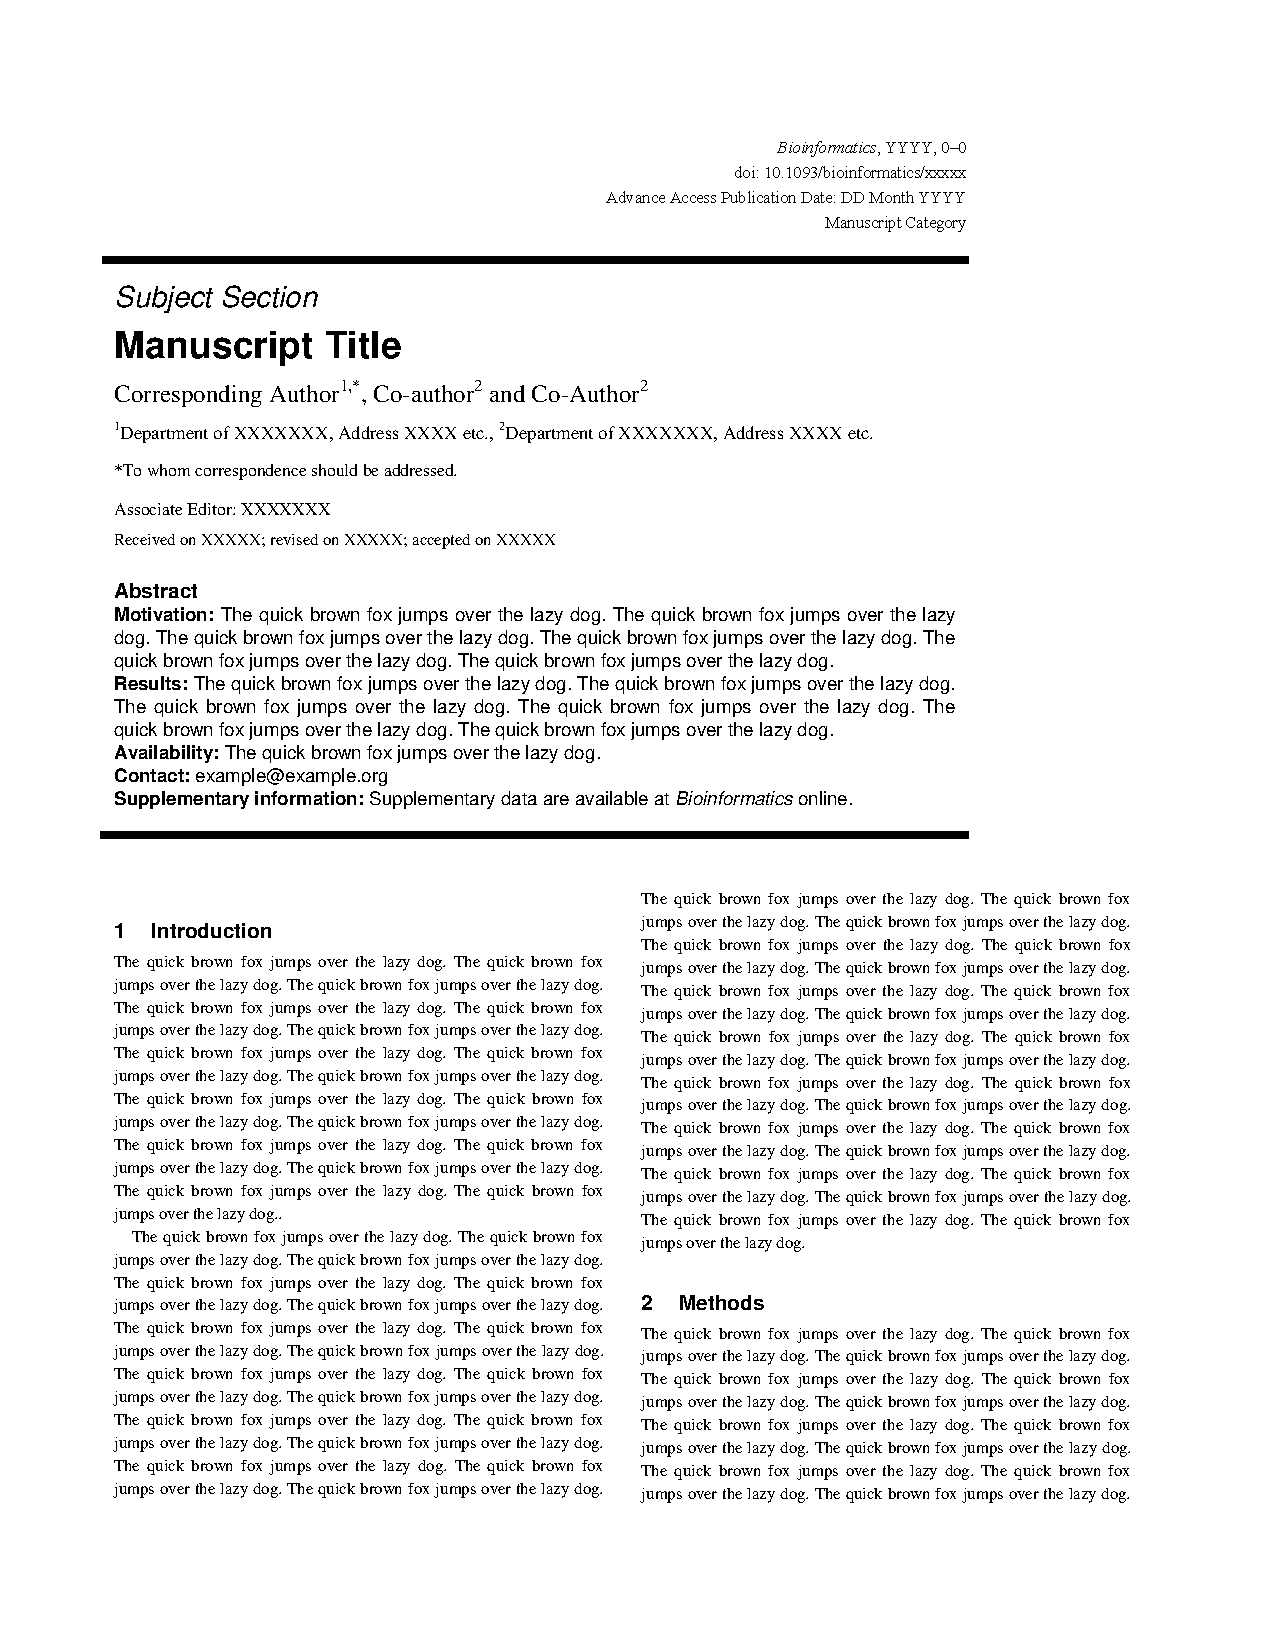
\includegraphics[width=0.8\textwidth, trim=0 15 0 0, clip]{images/Sample.pdf}
  \caption{A sample from PersonaMovs, which includes full modality data along with timestamps, personality label, relationship label, and personality vote distribution.}
  \label{fig:sample}
\end{figure*}


